\section{Software} \label{sec:software} 

This section starts with a justification of why we choose Julia to 
implement the GSVD algorithm described in section \ref{alg}. 
Then we discuss the design of the interface, and implementation details. 
Finally, we list the GSVD available in other 
programming languages. 

\subsection{Why Julia}

\paragraph{Two-language problem.}
There long exists a ``two-language'' problem programming language designers 
and software developers need to face: they have to make a trade-off 
when designing or choosing a language -- it can either be relatively 
easy for humans to write as a dynamic language, or relatively easy for 
computers to run as a statically-typed language, 
but not both \cite{perkel2019julia}.

When it comes to the realm of numerical and scientific computing, 
the first language Fortran \cite{10.5555/541529} dated back to 1957. Over six decades, 
the landscape of computing has changed dramatically due to the 
advance of hardware, algorithms, and tremendous increased amount of data, 
among others. An unfortunate outcome is that the most challenging areas 
of scientific computing have benefited the least from the enhanced 
abstraction and productivity offered by higher-level languages. 
Modern scientific computing environments such as 
Python (Numpy)~\cite{van2011numpy}, 
R~\cite{ihaka1996r}, 
Mathematica~\cite{math}, and 
MATLAB~\cite{MATLAB}, to name a few, 
have grown in popularity, all of which are weakly or dynamically typed. 
Still, when it comes to performance, none of these favored languages 
can compete against Fortran and C for solving computationally intensive problems
because weakly or dynamically typed language needs type check for variables, statement, field,
and even object and class hierarchy at runtime \cite{bezanson2017julia}. 

\paragraph{Julia -- introduction.} 
Julia is a new programming language that aims to address 
the ``two-language'' problem as its design philosophy lies in the combination of productivity 
and performance \cite{bezanson2017julia} \cite{edelman2019julia}.
By making use of JIT compilation, design paradigms such as
type inference, code specialization, and multiple dispatch,
Julia can generate optimized native 
code for multiple architectures and can approach the speed of Fortran and C \cite{Sengupta2019}. 
On top of that, Julia allows programmers to write high-level, generic and 
abstract code that closely resembles mathematical formulas. 

\paragraph{Julia -- features that we're particularly interested in.} ~ 
\begin{enumerate} 
\item {\bf A powerful approach to linear algebra.}

In addition to (and as part of) its support for multi-dimensional arrays, Julia provides native implementations for many linear algebra operations in the \texttt{LinearAlgebra} module. Basic matrix operations are implemented with calls to BLAS and LAPACK routines; the default implementation is OpenBLAS. 
Matrices with special symmetries and structures arise often in linear algebra and are frequently associated with various matrix factorizations. Julia features a rich collection of special matrix types, which allow for fast computation with specialized routines that are specially developed for particular matrix types. Optimization efforts are also made in compact storage. For instance, QR decomposition may return a ``thin'' \texttt{R} matrix, which is stored in a compact blocked format. Furthermore, Julia users can easily write user-extensible wrappers for BLAS and LAPACK on top of the \texttt{LinearAlgebra} library. LAPACK wrappers are implemented fully in Julia code, using \texttt{ccall}, which does not require a C compiler. 

For example, in linear algebra, MATLAB programmers may first find Julia more friendly because the array index in Julia also starts at 1, not 0. Those who are familiar with MATLAB functions should quickly adapt new adventure in Julia. The table below summarizes a list of Julia commands for frequently used matrix decompositions, and their counterparts in MATLAB. 

\begin{table}[H]
\centering
\scalebox{0.65}{
\begin{tabular}{|| c | c | c ||} \hline
Julia command & MATLAB command & Description \\ [0.5ex] \hline\hline
\texttt{schur(A::StridedMatrix) -> F::Schur} & \texttt{T = schur(A)} & Schur decomposition \\ \hline
         \texttt{lu(A, pivot=Val(true); check = true) -> F::LU} & \texttt{[L,U] = lu(A)} & LU decomposition \\ \hline
         \texttt{qr(A, pivot=Val(false)) -> F} & \texttt{[Q,R] = qr(A)} & QR decomposition \\ \hline
         \texttt{eigen(A; permute::Bool=true, scale::Bool=true, sortby) -> Eigen} & \texttt{[V,D] = eig(A)} & Eigenvalues and eigenvectors \\ \hline
         \texttt{svd(A; full::Bool = false) -> SVD} & \texttt{[U,S,V] = svd(A)} & Singular value decomposition \\
         \hline\hline
        \end{tabular}
}
\caption{Interfaces of commonly used matrix decompositions 
in Julia and MATLAB} \label{freq-decomp}
\end{table}

\item {\bf Ease-of-use.} 

MATLAB users may find a smooth transition to Julia as a fair amount of syntax of Julia are similar to that of MATLAB, if not the same. To begin with, both Julia and MATLAB use $\texttt{end}$ keyword to indicate code block. What's more, thanks to the magic of multiple dispatch, Julia brings ease of use to its programmers. Multiple dispatch is an unconventional object-oriented programming technique which allows users to depart from the limitations of class-based designs and instead leverage the expressive power of generic functions. For instance, elementary operations are intuitive, as simple as math. In that sense, users need not worry about the specific properties of numbers or matrices, the compilers will decide which specific algorithm should be used to take full advantage of the properties of the input data type.

\begin{table}[H]
\centering
\begin{tabular}{|| c | c | c ||} \hline
Operator & Function & Operand \\ [0.5ex] \hline\hline
\texttt{+} & add numbers/vectors/matrices & 
\makecell{\texttt{Int, Float, Vector, }\\ 
\texttt{Abstract Matrix, Dense Matrix, $\cdots$}} \\ \hline
\texttt{*} & multiply scale or compose & \texttt{Number, Function} \\ 
\hline\hline
\end{tabular}
\label{add-mul}
\end{table}

\item {\bf Speed.}  
 
Researchers and developers may first adopt Julia for its syntax, but they stay in the Julia community thanks to its speed. Some may think Julia is fast solely because it is Just-In-Time (JIT) 
compiled (i.e. every statement is run using compiled functions 
which are either compiled right before they are used, or cached compilations 
from before). However, other scripting languages Python, R, and MATLAB 
also use JIT, some by default. This leads to the question that what makes 
the key difference between Julia and other scripting languages 
in terms of speed?

The core design decision, type-stability through specialization via multiple-dispatch is what allows Julia to be very easy for a compiler to make into efficient code, but also allow the code to be very concise and ``look like a scripting language''. This will lead to some very clear performance gains. Multiple dispatch is functions are defined on different combinations of argument types, and applied by dispatching to the most specific matching definition. This model is a good fit for mathematical programming. If a function is type-stable, then the compiler can know what the type will be at all points in the function and smartly optimize it to the same assembly as C/Fortran.

\end{enumerate} 

\subsection{Interfaces of GSVD in Julia}

The output of the GSVD algorithm consists of six matrices and two integers. 
To follow Julia's convention as an object-oriented language, we encapsulate 
all the output into a composite type named \texttt{GeneralizedSVD}. 
In this way, users do not need to explicitly enumerate every matrix 
or integer in the return statement. In addition, doing so will facilitate 
those who only want to access part of the output. 
Hence, we define the composite type as a {\tt struct}. 

%\begin{lstlisting}[language=julia, style=jlcodestyle]
\begin{verbatim} 
struct GeneralizedSVD{T} <: Factorization{T}
    U::AbstractMatrix{T}
    V::AbstractMatrix{T}
    Q::AbstractMatrix{T}
    C::AbstractMatrix{T}
    S::AbstractMatrix{T}
    k::Int
    l::Int
    R::AbstractMatrix{T}
end
\end{verbatim} 
%\end{lstlisting}

Functions in Julia, particularly in ``\texttt{LinearAlgebra}'' package, 
are two-fold: one makes a copy of the input matrices or vectors, which
is convenient for testing purposes and is suitable for small inputs; 
the other overwrites the inputs in-place to save space and reduce communication overhead
between memory and cache. 

We adopt \Red{the practice of multiple dispatch} when designing the interface 
of the GSVD. This enables SVD of one matrix and GSVD of a matrix pair 
to share a single interface with different number or types of 
input arguments. Multiple dispatch allows a function to be written 
generically and thus maintains the language's expressiveness. 

\bigskip

Therefore, we provide two interfaces for the GSVD.  
%\begin{lstlisting}[language=julia, style=jlcodestyle]
\begin{verbatim} 
        svd(A, B) -> GeneralizedSVD
\end{verbatim} 
%\end{lstlisting}
or
%\begin{lstlisting}[language=julia, style=jlcodestyle]
\begin{verbatim} 
        svd!(A, B) -> GeneralizedSVD
\end{verbatim} 
%\end{lstlisting}


For both interfaces, compute the generalized SVD of \texttt{A} and \texttt{B},
returning a \texttt{GeneralizedSVD} object \texttt{F}, 
such that 
\begin{center} 
\texttt{A = F.U*F.C*F.R*F.Q'} 
\quad and \quad 
\texttt{B = F.V*F.S*F.R*F.Q'}. 
\end{center} 
For an \texttt{m}-by-\texttt{n} matrix \texttt{A} and \texttt{p}-by-\texttt{n} matrix \texttt{B},
\begin{itemize}
\item \texttt{U} is an \texttt{m}-by-\texttt{m} orthogonal matrix,
\item \texttt{V} is a \texttt{p}-by-\texttt{p} orthogonal matrix,
\item \texttt{Q} is an \texttt{n}-by-\texttt{n} orthogonal matrix,
\item \texttt{C} is an \texttt{m}-by-\texttt{(k+l)} diagonal matrix with 1s in the first K entries,
\item \texttt{S} is a \texttt{p}-by-\texttt{(k+l)} matrix whose top right \texttt{l}-by-\texttt{l} block is diagonal,
\item \texttt{R} is a \texttt{(k+l)}-by-\texttt{n} matrix whose rightmost \texttt{(k+l)}-by-\texttt{(k+l)} block is nonsingular upper block triangular,
\item \texttt{k+l} is the effective numerical 
rank of the matrix \texttt{[A; B]}. One can get {\tt k+l}
from {\tt F.k + F.l} 
\end{itemize}

\texttt{svd!} is the same as \texttt{svd}, but modifies the 
arguments \texttt{A} and \texttt{B} in-place, instead of making copies. 

On exit,
\begin{enumerate}
	\item If $m-k-\ell \geq 0$
		\begin{equation*}
			R = \bordermatrix{ 
               & n-k-\ell & k + \ell \cr
    			\hfill k+\ell & 0 & R_{0} \cr}
		\end{equation*}
		$R_{0}$ is stored in \texttt{A[1:k+l,n-k-l+1:n]}.
	\item If $m-k-\ell <0$
		\begin{equation*}
			R = \bordermatrix{ 
               & n-k-\ell & k & m-k & k+\ell-m \cr
               \hfill k & 0 & R_{11} & R_{12} & R_{13} \cr
    			\hfill m-k & 0 & 0 & R_{22} & A_{23} \cr
    			\hfill k+\ell-m & 0 & 0 & 0 & R_{33} \cr}
		\end{equation*}
		$\begin{pmatrix}
			R_{11} & R_{12} & R_{13} \\
			0 & R_{22} & R_{23}
		\end{pmatrix}$
		is stored in \texttt{A[1:m, n-k-l+1:n]} and $R_{33}$ is stored in 
		\texttt{B[m-k+1:l,n+m-k-l+1:n]}.
\end{enumerate}


\subsection{GSVD module and implementation details}

The structural unit called \texttt{Module} is native in Julia to 
group relevant functions and definitions. 

The main module of the GSVD algorithm is \texttt{GSVD}. 
In addition, considering that the safe diagonalization not only serves 
as a building block for the GSVD algorithm, but is also a 
tool in other applications, we have separated the safe diagonalization 
as a stand alone module called \texttt{SafeDiag}. 

The architecture of the GSVD implemention 
is shown in the following UML class diagram.  % in Figure~\ref{uml-class}. 
%\begin{figure}%[H]
\begin{center} 
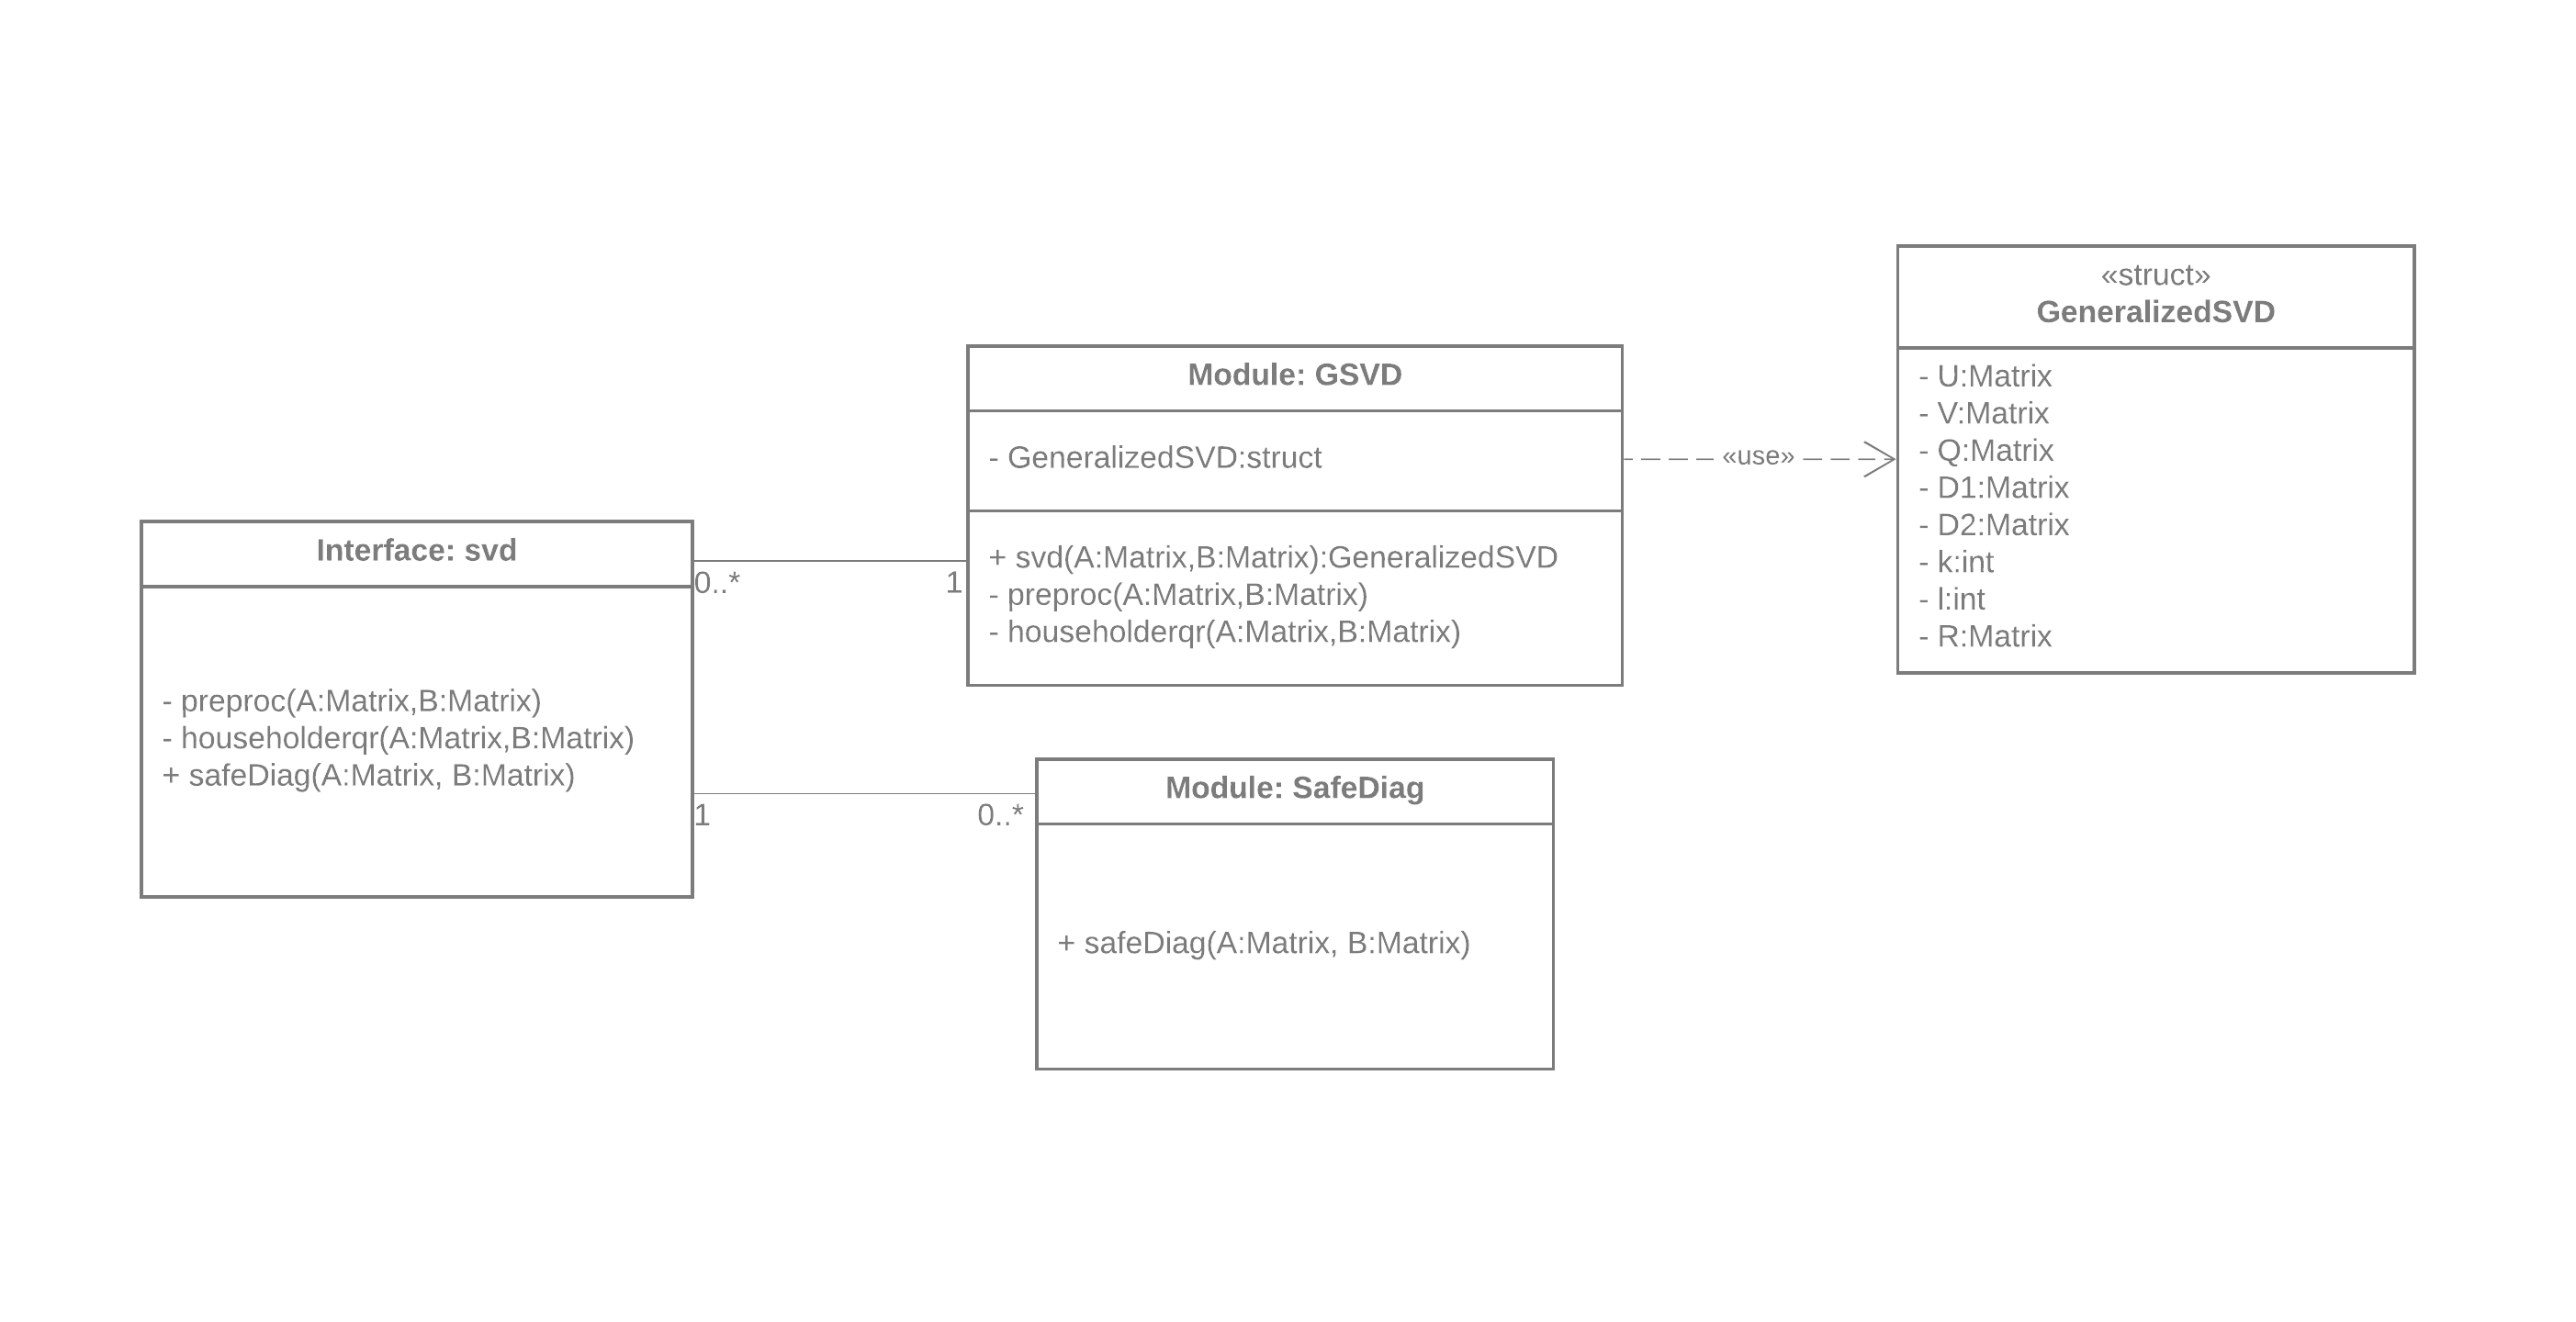
\includegraphics[width=0.75\linewidth]{fig/GSVD_class.png}
\end{center} 
%\caption{UML class diagram for the GSVD} \label{uml-class}
%\end{figure}

The GSVD algorithm starts from the main function \texttt{svd()} 
under module \texttt{GSVD}. It then calls \texttt{preproc()}. 
Once return, it calls function \texttt{safeDiag} intermodularly. 
Finally, upon return, the main function post-processes to 
formulate the outputs. The sequence of the major function 
calls is the following. 

\begin{center}
\fbox{\texttt{GSVD:svd()}} $\rightarrow$ 
\fbox{\texttt{GSVD:preproc()}} $\rightarrow$ 
\fbox{\texttt{GSVD:householderqr()}} $\rightarrow$ 
\fbox{\texttt{SafeDiag:safediag}}
\end{center}

The details of each major functions are discussed below. 
\begin{itemize} 
\item \fbox{\texttt{GSVD:preproc()}}

    This step is to reduce two input matrices $A$ and $B$ into two upper triangular forms. This is done via a call to \texttt{preproc()}. This function makes use of three fundamental orthogonal decompositions. 
    \begin{enumerate}
    	\item First is QR decomposition with column pivoting to reveal the numerical rank of $B$ and $[A; B]$ without forming the matrix explicitly. This is done by a call to \texttt{qr(A, pivot=Val(true)))}. Let \texttt{tolB} as the tolerance to determine the effective rank of $B = \ell$.
		\begin{equation*}
			tol_{B} = max\{p, n\}\Vert B \Vert_1 \epsilon
		\end{equation*}
		where $\epsilon$ is the machine precision of \texttt{Float64}. \\
		We also use QR decomposition with column pivoting again on the leftmost $n-\ell$ columns of $A$. Similarly, by defining
		\begin{equation*}
			tol_{A} = max\{m, n\}\Vert A \Vert_1 \epsilon
		\end{equation*}
		we compute the effective rank of $[A; B] = k+ \ell$.
		\item Second is RQ decomposition of the top $\ell$ rows of $B$ if $n > \ell$ via a call to \texttt{LAPACK.gerqf!()}. It is called a second time on $A$ if $n - \ell > k$.
		\item Third is QR decomposition of $A$ when $m > k$ by calling \texttt{qr()}. 
	\end{enumerate}
	Upon return to \texttt{svd()}, two of the upper triangular matrices overwrites $A$ and $B$, the orthogonal matrices are placed in U, V, and Q and rank information is stored in $k$ and $\ell$.

\item \fbox{\texttt{GSVD:householderqr()}} 
    
    This step is to reduce two upper triangular matrices to one and is done by calling \texttt{householderqr()}. On entry, two triangular matrices are stacked together and passed as the arguments of \texttt{qr()}. On exit, $Q_1$ and $Q_2$ overwrites inputs.  
    
\item \fbox{\texttt{SafeDiag:safediag}}
    
    This step calls \texttt{safeDiag()} from module \texttt{SafeDiag}. This function requires SVD, and QR decomposition. This is done by calls to \texttt{svd()}, \texttt{qr()} respectively. 
    \begin{enumerate}
    	\item We first compute SVD of $Q_{2}$. To preserve the order of $\{\cos\theta\}$, we have to reverse the order of the singular values of $Q_{2}$. 
		\item Since $\{\cos\theta\}$ are already sorted, we take advantage of binary search to find the threshold $r$.
		\item QR decomposition of the multiply of $Q_{1}$ and right singular vectors of $Q_{2}$. $R$ is not only triangular but diagonal. However, sanitization is necessary to assure the non-negativity of the diagonal entries. 
    \end{enumerate}
    
    It return $U_1, V_1, Z_1, C, S$ on exit.   

\item Post-processing:

    In this step, we update matrix $U$, $V$ and $Q$ by matrix-matrix multiply. To formulate $R$, we utilize RQ decomposition via a call to \texttt{LAPACK.gerqf!()}. Finally, we put matrices $U, V, C, S, Q$ and $k$, $\ell$ into the constructor of \texttt{GeneralizedSVD} as return. 

\end{itemize}
We implement the GSVD algorithm in Julia 1.3 using \texttt{Float64} data. 


\subsection{Lessons and caveats} 
We capture some pitfalls that might be a bottleneck, 
and thus are worth mentioning.
\begin{itemize} 

\item {\bf Some inconsistent interface design.}

As a modern programming language, Julia supports multiple dispatch, that is, parametric polymorphism. A good example is that the GSVD interface reuses the name of the SVD of a single matrix $A$ by taking two matrices as arguments. Unfortunately, this principle is not fully implemented. For instance, when computing the matrix norm, one may intuitively call \texttt{norm(A)}. However, this will not produce the desired result as shown below. Instead, one may want to use \texttt{opnorm(A)}. 

\begin{table}[H]
\centering
\begin{tabular}{|| c | c ||} \hline
Julia command/result & MATLAB command/result\\ [0.5ex] \hline\hline
\makecell{\texttt{norm([1 2 3; 4 5 6; 7 8 9])} \\
16.881943016134134} & \makecell{\texttt{norm([1 2 3;4 5 6;7 8 9])} \\ 16.8481} \\
\hline\hline
\makecell{\texttt{opnorm([1 2 3; 4 5 6; 7 8 9])} \\
16.84810335261421} & N/A \\
\hline\hline
\end{tabular}
\label{norm-api}
\end{table}

\item {Performance relies on ``proper'' implementation.}

Our GSVD algorithm involves many operations with submatrices. We don't need to pay attention to matrix slicing in other languages. However, in Julia, this could be a significant performance issue since slicing an array creates a copy of the selected subarray, which is computational expensive.  
To make things worse, if a sliced matrix is passed as the return value, the result will be inaccurate as it is not overwritten in the original matrix. 

An alternative is to create a ``view'' of the array, which is an array object that actually references the data of the original array in-place, without making a copy. This can be done for individual slices by calling function \texttt{view}, or more simply for a whole expression or block of code by putting macro \texttt{@views} in front of that expression. One can tell from the following example that by doing so, the speedup is three-fold. 

%\begin{lstlisting}[language=julia, style=jlcodestyle]
\begin{verbatim}
	julia> fcopy(x) = sum(x[2:end-1]);
	julia> @views fview(x) = sum(x[2:end-1]);
	julia> x = rand(10^6);
	julia> @time fcopy(x);
  	0.003051 seconds (7 allocations: 7.630 MB)
	julia> @time fview(x);
  	0.001020 seconds (6 allocations: 224 bytes)
\end{verbatim}
%\end{lstlisting}

\end{itemize} 

Many other features of Julian have not been studied and explored 
by the author, most notably, parallelism. This could be 
a good direction for future work. 


\subsection{GSVD in other languages}  
A number of numerical computing platforms feature 
the GSVD is listed in the following table. 
%Table \ref{tab:gsvdlang} is a list of ones we know of. 
    
%\begin{table}%[H]
%\centering
\begin{center} 
\scalebox{0.80}{
\begin{tabular}{|c|c|} \hline
Language & GSVD Documentation \\ \hline\hline
            Native Julia (proposed) &  \makecell[l]{\texttt{svd(A, B) -> GeneralizedSVD} \\ Computes the generalized SVD of \texttt{A} and \texttt{B},  returning a \texttt{GSVD} factorization\\ object \texttt{F}, such that \\ \texttt{A = F.U*F.C*F.R*F.Q'} and \texttt{B = F.V*F.S*F.R*F.Q'}.}\\ \hline
            Julia 1.3 (LAPACK wrapper) &  \makecell[l]{\texttt{svd(A, B) -> GeneralizedSVD} \\ Computes the generalized SVD of \texttt{A} and \texttt{B},  returning a \texttt{GeneralizedSVD}\\ factorization object \texttt{F}, such that \\ \texttt{A = F.U*F.D1*F.R0*F.Q'} and \texttt{B = F.V*F.D2*F.R0*F.Q'}.}\\ \hline
            MATLAB (2019b) & \makecell[l]{\texttt{[U,V,X,C,S] = gsvd(A,B)} \\
            Returns unitary matrices \texttt{U} and \texttt{V}, a (usually) square matrix \texttt{X}, and \\ nonnegative diagonal matrices \texttt{C} and \texttt{S} so that \\
                \texttt{A = U*C*X', B = V*S*X', C'*C + S'*S = I}.}\\ \hline
            Mathematica & \makecell[l]{\texttt{SingularValueDecomposition[{m,a}]} \\
            Gives a list of matrices \{\texttt{{u,ua},{w,wa},v}\} such that \texttt{m} can be written as \\ \texttt{u.w.Conjugate[Transpose[v]]} and \texttt{a} can be written as \\ \texttt{ua.wa.Conjugate[Transpose[v]]}. } \\ \hline
            R (geigen v2.3, LAPACK wrapper) & \makecell[l]{\texttt{z <- gsvd(A, B)}\\
            Computes The Generalized Singular Value Decomposition of matrices \\ $A$ and $B$ such that $A = UD_{1}[0 \ R]Q^{T}$ and $B = VD_{2}[0 R]Q^{T}$. Note that \\ the return value is the same as the output of LAPACK 3.6 and above. }
            \\\hline
            Python (R. Luo's thesis) &  \makecell[l]{Didn't disclose API design. The author defined GSVD as follows: \\
            Given two $M_i$-by-$N$ column-matched but row-independent matrices $D_{i}$, \\ each with full column rank and $N \leq Mi$, the GSVD is an exact \\ simultaneous factorization $Di = Ui \Sigma_i V^T, i = 1, 2$. $U_i$ is $M_i$-by-$N$ and \\ are column-wise orthonormal and $V$ is $N$-by-$N$ nonsingular matrix with\\ normalized rows. $diag(\Sigma_i)$ returns two lists of $N$ positive values and \\the ratios are called the generalized singular values.} \\ \hline
        \end{tabular}
} 
\end{center} 
% \caption{GSVD in different languages} \label{tab:gsvdlang}
%\end{table}
